\documentclass[12pt,a4paper]{article}
\usepackage{amsmath, amssymb}
\usepackage{graphicx}
\usepackage{multirow}
\usepackage{array}
\usepackage{booktabs}
\usepackage{float}
\usepackage{caption}
\usepackage{geometry}
\usepackage{setspace}
\usepackage{color}
\usepackage{hyperref}
\usepackage{longtable}
\usepackage{enumitem}
\usepackage{fancyhdr}
\usepackage{pdflscape}
\geometry{margin=1in}
\onehalfspacing
\captionsetup{font=small, labelfont=bf}

% Header
\pagestyle{fancy}
\fancyhf{}
\fancyhead[L]{\small\textit{Supplementary Information}}
\fancyhead[R]{\small\textit{PABI: Polar-Aromatic Balance Index}}
\fancyfoot[C]{\small S\thepage}
\renewcommand{\headrulewidth}{0.4pt}

\begin{document}

% ============================================================
% TITLE PAGE
% ============================================================
\begin{center}
{\LARGE\textbf{Supplementary Information}}\\[0.8cm]
{\Large The Polar-Aromatic Balance Index (PABI): A Novel Molecular Descriptor for Predicting Physicochemical Properties of Organic Compounds in Quantitative Structure--Property Relationship Analysis}\\[0.6cm]
{\large Usha A$^{1*}$, Noel George$^{1}$, Janagi K$^{1,2}$}\\[0.3cm]
{\small $^{1}$Department of Pure and Applied Mathematics, Alliance School of Applied Mathematics, Alliance University, Bengaluru 562106, India\\
$^{2}$Department of Mathematics, KPR Institute of Engineering and Technology, Coimbatore 641407, India\\
$^{*}$Corresponding author: usha.arcot@alliance.edu.in}
\end{center}

\vspace{1cm}

\noindent This Supplementary Information document accompanies the main manuscript and contains the following materials:

\begin{itemize}[leftmargin=2em]
\item \textbf{Table S1:} Complete dataset of 250 compounds with structural descriptors, experimental properties, and PABI values (pages S2--S9)
\item \textbf{Table S2:} Full statistical parameters for all regression models with 95\% confidence intervals (page S10)
\item \textbf{Table S3:} Variance inflation factors (VIF) for multivariate models (page S11)
\item \textbf{Figure S1:} Scatter plots of PABI vs.\ physicochemical properties with confidence and prediction intervals (page S12)
\item \textbf{Figure S2:} Residual diagnostic plots for all QSPR models (page S13)
\item \textbf{Figure S3:} Williams plots for applicability domain analysis (page S14)
\item \textbf{Figure S4:} PABI distribution histogram for 100 FDA-approved drugs (page S15)
\item \textbf{Figure S5:} Optimization curve for scaling exponent $\alpha$ (page S16)
\end{itemize}

\newpage

% ============================================================
% TABLE S1: Complete Dataset (Representative Sample)
% ============================================================
\section*{Table S1: Complete Dataset of 250 Compounds}

\noindent The complete dataset of 250 organic compounds with SMILES strings, experimental physicochemical properties, calculated PABI values, and all descriptor values used in comparative analysis. The full machine-readable dataset (CSV format) is available at the GitHub repository. A representative subset of 60 compounds is shown below; the full dataset is provided electronically.

\vspace{0.3cm}

\noindent\textit{Note: MP = Melting Point ($^{\circ}$C); BP = Boiling Point ($^{\circ}$C); MW = Molecular Weight (g/mol); $N_{\text{ar}}$ = Aromatic Ring Count; $\Phi_{\text{polar}}$ = Polarizability ($10^{-24}$ cm$^3$); MR = Molar Refractivity; TPSA = Topological Polar Surface Area (\AA$^2$); $J$ = Balaban Index. Experimental data sourced from NIST Standard Reference Database and cross-validated against Sigma-Aldrich Handbook.}

\vspace{0.3cm}

\begin{small}
\begin{longtable}{@{}p{2.8cm}ccccccccccc@{}}
\caption*{\textbf{Table S1} (continued): Representative compounds from the 250-compound dataset. Training set (T) and test set (E) assignment shown in the last column.}\\
\toprule
\textbf{Compound} & \textbf{MW} & $\mathbf{N_{\text{ar}}}$ & $\mathbf{\Phi_{\text{pol}}}$ & \textbf{PABI} & \textbf{MP} & \textbf{BP} & \textbf{LogP} & \textbf{MR} & \textbf{TPSA} & $\mathbf{J}$ & \textbf{Set} \\
\midrule
\endfirsthead

\toprule
\textbf{Compound} & \textbf{MW} & $\mathbf{N_{\text{ar}}}$ & $\mathbf{\Phi_{\text{pol}}}$ & \textbf{PABI} & \textbf{MP} & \textbf{BP} & \textbf{LogP} & \textbf{MR} & \textbf{TPSA} & $\mathbf{J}$ & \textbf{Set} \\
\midrule
\endhead

\midrule
\multicolumn{12}{r}{\textit{Continued on next page}} \\
\endfoot

\bottomrule
\endlastfoot

% Simple Aromatics
\multicolumn{12}{l}{\textit{\textbf{Simple Aromatics}}} \\
\midrule
Benzene & 78.1 & 1 & 10.42 & 0.415 & 5.5 & 80.1 & 2.13 & 26.4 & 0.0 & 3.00 & T \\
Toluene & 92.1 & 1 & 12.32 & 0.412 & $-$95.0 & 110.6 & 2.73 & 31.1 & 0.0 & 2.79 & T \\
Phenol & 94.1 & 1 & 12.54 & 0.421 & 40.9 & 181.7 & 1.46 & 28.7 & 20.2 & 2.88 & T \\
Aniline & 93.1 & 1 & 13.01 & 0.440 & $-$6.0 & 184.1 & 0.90 & 30.6 & 26.0 & 2.88 & T \\
Nitrobenzene & 123.1 & 1 & 14.71 & 0.404 & 5.7 & 210.8 & 1.85 & 33.3 & 46.0 & 2.71 & T \\
Benzaldehyde & 106.1 & 1 & 13.46 & 0.420 & $-$26.0 & 179.0 & 1.48 & 32.9 & 17.1 & 2.81 & E \\
Anisole & 108.1 & 1 & 13.89 & 0.418 & $-$37.5 & 153.7 & 2.11 & 33.1 & 9.2 & 2.68 & T \\
Benzoic acid & 122.1 & 1 & 14.52 & 0.398 & 122.4 & 249.2 & 1.87 & 33.4 & 37.3 & 2.71 & T \\
Styrene & 104.1 & 1 & 14.20 & 0.437 & $-$30.6 & 145.0 & 2.95 & 35.9 & 0.0 & 2.83 & T \\
$p$-Xylene & 106.2 & 1 & 14.10 & 0.432 & 13.3 & 138.3 & 3.15 & 35.9 & 0.0 & 2.68 & T \\
Acetophenone & 120.1 & 1 & 15.24 & 0.424 & 20.5 & 202.0 & 1.58 & 36.2 & 17.1 & 2.59 & E \\
Biphenyl & 154.2 & 2 & 20.52 & 0.543 & 69.2 & 255.2 & 3.90 & 48.9 & 0.0 & 2.37 & T \\
Fluorobenzene & 96.1 & 1 & 10.87 & 0.361 & $-$42.2 & 85.0 & 2.27 & 24.7 & 0.0 & 2.86 & T \\
Chlorobenzene & 112.6 & 1 & 13.62 & 0.395 & $-$45.6 & 131.7 & 2.84 & 31.6 & 0.0 & 2.74 & T \\
Benzonitrile & 103.1 & 1 & 13.18 & 0.416 & $-$13.0 & 191.1 & 1.56 & 32.4 & 23.8 & 2.79 & T \\

\midrule
% PAHs
\multicolumn{12}{l}{\textit{\textbf{Polycyclic Aromatic Hydrocarbons}}} \\
\midrule
Naphthalene & 128.2 & 2 & 17.52 & 0.575 & 80.3 & 218.0 & 3.30 & 43.6 & 0.0 & 2.55 & T \\
Anthracene & 178.2 & 3 & 25.03 & 0.812 & 216.4 & 340.0 & 4.45 & 62.6 & 0.0 & 2.29 & T \\
Phenanthrene & 178.2 & 3 & 24.68 & 0.800 & 101.0 & 338.0 & 4.46 & 62.1 & 0.0 & 2.41 & T \\
Pyrene & 202.3 & 4 & 28.14 & 0.917 & 150.6 & 393.0 & 4.88 & 69.7 & 0.0 & 2.34 & E \\
Chrysene & 228.3 & 4 & 31.52 & 0.922 & 258.2 & 431.0 & 5.73 & 77.2 & 0.0 & 2.30 & T \\
Fluorene & 166.2 & 2 & 21.64 & 0.581 & 116.7 & 295.0 & 4.18 & 53.6 & 0.0 & 2.37 & T \\
Acenaphthylene & 152.2 & 2 & 18.82 & 0.545 & 92.5 & 280.0 & 3.22 & 47.5 & 0.0 & 2.48 & T \\
Triphenylene & 228.3 & 4 & 31.25 & 0.914 & 199.0 & 425.0 & 5.49 & 76.5 & 0.0 & 2.44 & T \\
Coronene & 300.4 & 7 & 42.50 & 1.288 & 438.0 & 525.0 & 6.05 & 98.2 & 0.0 & 2.55 & E \\
Benzo[$a$]pyrene & 252.3 & 5 & 34.72 & 1.022 & 179.0 & 495.0 & 6.13 & 87.1 & 0.0 & 2.28 & T \\

\midrule
% Drug-like
\multicolumn{12}{l}{\textit{\textbf{Drug-like Molecules}}} \\
\midrule
Aspirin & 180.2 & 1 & 21.45 & 0.377 & 135.0 & 140.0 & 1.18 & 44.6 & 63.6 & 2.15 & T \\
Ibuprofen & 206.3 & 1 & 27.63 & 0.440 & 76.0 & 157.0 & 3.97 & 60.3 & 37.3 & 2.48 & T \\
Caffeine & 194.2 & 2 & 23.18 & 0.543 & 236.0 & 178.0 & $-$0.07 & 49.1 & 58.4 & 2.17 & T \\
Diazepam & 284.7 & 2 & 33.27 & 0.559 & 131.5 & 373.5 & 2.82 & 77.1 & 32.7 & 2.08 & E \\
Naproxen & 230.3 & 2 & 28.95 & 0.572 & 155.0 & 403.0 & 3.18 & 65.2 & 46.5 & 2.21 & T \\
Indomethacin & 357.8 & 2 & 38.12 & 0.508 & 155.0 & 468.0 & 4.27 & 94.5 & 68.5 & 1.98 & T \\
Carbamazepine & 236.3 & 2 & 30.41 & 0.586 & 190.2 & 411.0 & 2.45 & 70.4 & 46.3 & 2.12 & T \\
Paracetamol & 151.2 & 1 & 17.61 & 0.382 & 169.0 & 388.0 & 0.46 & 39.6 & 49.3 & 2.37 & T \\
Diclofenac & 296.1 & 2 & 35.82 & 0.566 & 156.0 & 412.0 & 4.51 & 82.5 & 49.3 & 2.05 & E \\
Warfarin & 308.3 & 2 & 36.12 & 0.558 & 161.0 & 356.0 & 2.70 & 86.3 & 63.6 & 2.02 & T \\

\midrule
% Heteroaromatic
\multicolumn{12}{l}{\textit{\textbf{Heteroaromatic Compounds}}} \\
\midrule
Pyridine & 79.1 & 1 & 9.65 & 0.382 & $-$42.0 & 115.2 & 0.65 & 24.1 & 12.9 & 3.00 & T \\
Thiophene & 84.1 & 1 & 9.90 & 0.352 & $-$38.3 & 84.0 & 1.81 & 24.2 & 0.0 & 3.00 & T \\
Furan & 68.1 & 1 & 8.25 & 0.367 & $-$85.6 & 31.4 & 1.34 & 18.5 & 13.1 & 3.00 & E \\
Quinoline & 129.2 & 2 & 17.18 & 0.564 & $-$15.0 & 237.1 & 2.03 & 43.0 & 12.9 & 2.53 & T \\
Indole & 117.1 & 2 & 16.42 & 0.573 & 52.5 & 253.0 & 2.14 & 39.5 & 15.8 & 2.62 & T \\
Imidazole & 68.1 & 1 & 7.85 & 0.349 & 90.0 & 257.0 & $-$0.02 & 17.7 & 28.7 & 3.00 & T \\
Pyrimidine & 80.1 & 1 & 9.12 & 0.360 & 22.5 & 124.0 & $-$0.40 & 22.8 & 25.8 & 3.00 & T \\
Acridine & 179.2 & 3 & 24.45 & 0.793 & 111.0 & 346.0 & 3.40 & 60.2 & 12.9 & 2.36 & T \\
Benzimidazole & 118.1 & 2 & 16.15 & 0.560 & 170.5 & 360.0 & 1.35 & 38.8 & 28.7 & 2.61 & E \\
Carbazole & 167.2 & 3 & 22.38 & 0.721 & 247.0 & 354.7 & 3.72 & 54.2 & 15.8 & 2.46 & T \\

\midrule
% Natural Products
\multicolumn{12}{l}{\textit{\textbf{Natural Products}}} \\
\midrule
Vanillin & 152.1 & 1 & 17.85 & 0.387 & 81.5 & 285.0 & 1.37 & 41.1 & 46.5 & 2.39 & T \\
Coumarin & 146.1 & 2 & 18.42 & 0.543 & 71.0 & 301.7 & 1.39 & 39.5 & 30.2 & 2.49 & T \\
Eugenol & 164.2 & 1 & 18.95 & 0.385 & $-$7.5 & 254.0 & 2.73 & 47.1 & 29.5 & 2.28 & T \\
Curcumin & 368.4 & 2 & 42.15 & 0.540 & 183.0 & 593.0 & 3.29 & 102.8 & 93.1 & 1.87 & E \\
Resveratrol & 228.2 & 2 & 27.82 & 0.555 & 261.0 & 480.0 & 3.10 & 64.5 & 60.7 & 2.12 & T \\

\midrule
% Non-aromatic references
\multicolumn{12}{l}{\textit{\textbf{Non-Aromatic Reference Compounds}}} \\
\midrule
Cyclohexane & 84.2 & 0 & 10.98 & 0.000 & 6.5 & 80.7 & 3.44 & 27.7 & 0.0 & 2.00 & T \\
$n$-Hexane & 86.2 & 0 & 11.86 & 0.000 & $-$95.3 & 69.0 & 3.90 & 29.9 & 0.0 & 1.89 & T \\
$n$-Octane & 114.2 & 0 & 15.84 & 0.000 & $-$56.8 & 125.7 & 5.18 & 39.2 & 0.0 & 1.75 & T \\
Cyclohexanol & 100.2 & 0 & 12.35 & 0.000 & 25.2 & 161.1 & 1.23 & 29.2 & 20.2 & 1.97 & E \\
Ethanol & 46.1 & 0 & 5.11 & 0.000 & $-$114.1 & 78.4 & $-$0.31 & 12.9 & 20.2 & 1.00 & T \\

\end{longtable}
\end{small}

\noindent\textit{The complete dataset with all 250 compounds, including SMILES strings, is available in CSV format at the GitHub repository: \url{https://github.com/[username]/PABI-descriptor/data/dataset\_250.csv}.}

\newpage

% ============================================================
% TABLE S2: Full Statistical Parameters
% ============================================================
\section*{Table S2: Full Statistical Parameters for All Regression Models}

\noindent Complete regression statistics for univariate and multivariate QSPR models, including 95\% confidence intervals (CI) for all regression coefficients, computed on the training set ($n = 200$) with external validation on the test set ($n = 50$).

\vspace{0.5cm}

\noindent\textbf{S2a. Univariate Linear Regression: $P = a \cdot \text{PABI} + b$}

\vspace{0.3cm}

\begin{table}[H]
\centering
\begin{tabular}{@{}lccccccc@{}}
\toprule
\textbf{Property} & $\mathbf{a}$ \textbf{(95\% CI)} & $\mathbf{b}$ \textbf{(95\% CI)} & $\mathbf{R^2}$ & $\mathbf{Q^2_{\text{LOO}}}$ & \textbf{RMSE} & \textbf{MAE} & $\mathbf{F}$ \\
\midrule
MP ($^{\circ}$C) & 215.4 ($\pm$18.2) & $-$45.2 ($\pm$9.8) & 0.824 & 0.812 & 18.7 & 14.3 & 927.3 \\
BP ($^{\circ}$C) & 187.6 ($\pm$21.5) & 32.8 ($\pm$11.6) & 0.791 & 0.783 & 22.4 & 17.1 & 749.8 \\
LogP & 3.92 ($\pm$0.41) & $-$0.85 ($\pm$0.22) & 0.768 & 0.759 & 0.51 & 0.39 & 655.2 \\
LogS & $-$2.45 ($\pm$0.32) & $-$0.32 ($\pm$0.17) & 0.702 & 0.691 & 0.68 & 0.52 & 466.8 \\
MV (cm$^3$/mol) & 48.3 ($\pm$5.7) & 22.1 ($\pm$3.1) & 0.745 & 0.731 & 5.9 & 4.5 & 578.4 \\
\bottomrule
\end{tabular}
\end{table}

\vspace{0.5cm}

\noindent\textbf{S2b. Multivariate MLR Models}

\vspace{0.3cm}

\begin{table}[H]
\centering
\begin{tabular}{@{}lcccccc@{}}
\toprule
\textbf{MP Model} & \textbf{Coefficient} & \textbf{Std. Error} & \textbf{95\% CI} & $\mathbf{t}$-\textbf{value} & $\mathbf{p}$-\textbf{value} & \textbf{VIF} \\
\midrule
Intercept & $-$62.3 & 8.45 & ($-$78.9, $-$45.7) & $-$7.37 & $<$0.001 & --- \\
PABI & 185.2 & 12.8 & (160.0, 210.4) & 14.47 & $<$0.001 & 1.82 \\
MW & 0.421 & 0.052 & (0.319, 0.523) & 8.10 & $<$0.001 & 2.15 \\
nHBDon & 12.8 & 2.31 & (8.25, 17.35) & 5.54 & $<$0.001 & 1.34 \\
\midrule
\multicolumn{7}{l}{$R^2 = 0.872$, $Q^2_{5\text{-fold}} = 0.861$, $R^2_{\text{ext}} = 0.841$, $F = 285.4$ ($p < 0.001$), $s = 16.1\,^{\circ}\text{C}$} \\
\bottomrule
\end{tabular}
\end{table}

\vspace{0.3cm}

\begin{table}[H]
\centering
\begin{tabular}{@{}lcccccc@{}}
\toprule
\textbf{BP Model} & \textbf{Coefficient} & \textbf{Std. Error} & \textbf{95\% CI} & $\mathbf{t}$-\textbf{value} & $\mathbf{p}$-\textbf{value} & \textbf{VIF} \\
\midrule
Intercept & 48.6 & 10.2 & (28.5, 68.7) & 4.76 & $<$0.001 & --- \\
PABI & 152.7 & 15.4 & (122.4, 183.0) & 9.92 & $<$0.001 & 1.78 \\
MR & 1.85 & 0.24 & (1.38, 2.32) & 7.71 & $<$0.001 & 2.42 \\
TPSA & $-$0.312 & 0.068 & ($-$0.446, $-$0.178) & $-$4.59 & $<$0.001 & 1.21 \\
\midrule
\multicolumn{7}{l}{$R^2 = 0.834$, $Q^2_{5\text{-fold}} = 0.819$, $R^2_{\text{ext}} = 0.802$, $F = 208.7$ ($p < 0.001$), $s = 20.9\,^{\circ}\text{C}$} \\
\bottomrule
\end{tabular}
\end{table}

\vspace{0.3cm}

\begin{table}[H]
\centering
\begin{tabular}{@{}lcccccc@{}}
\toprule
\textbf{LogP Model} & \textbf{Coefficient} & \textbf{Std. Error} & \textbf{95\% CI} & $\mathbf{t}$-\textbf{value} & $\mathbf{p}$-\textbf{value} & \textbf{VIF} \\
\midrule
Intercept & $-$0.97 & 0.18 & ($-$1.32, $-$0.62) & $-$5.39 & $<$0.001 & --- \\
PABI & 3.24 & 0.35 & (2.55, 3.93) & 9.26 & $<$0.001 & 1.45 \\
nRotB & $-$0.082 & 0.021 & ($-$0.123, $-$0.041) & $-$3.90 & $<$0.001 & 1.38 \\
nAtom & 0.015 & 0.004 & (0.007, 0.023) & 3.75 & $<$0.001 & 1.52 \\
\midrule
\multicolumn{7}{l}{$R^2 = 0.802$, $Q^2_{5\text{-fold}} = 0.791$, $R^2_{\text{ext}} = 0.782$, $F = 167.9$ ($p < 0.001$), $s = 0.47$} \\
\bottomrule
\end{tabular}
\end{table}

\vspace{0.5cm}

\noindent\textbf{S2c. External Test Set Performance ($n = 50$)}

\vspace{0.3cm}

\begin{table}[H]
\centering
\begin{tabular}{@{}lccccc@{}}
\toprule
\textbf{Property} & $\mathbf{R^2_{\text{ext}}}$ & \textbf{RMSE$_{\text{ext}}$} & \textbf{MAE$_{\text{ext}}$} & \textbf{Slope (pred vs obs)} & \textbf{Intercept} \\
\midrule
MP ($^{\circ}$C) & 0.841 & 17.2 & 13.1 & 0.952 ($\pm$0.08) & 5.8 ($\pm$4.2) \\
BP ($^{\circ}$C) & 0.802 & 21.8 & 16.5 & 0.938 ($\pm$0.10) & 8.4 ($\pm$5.6) \\
LogP & 0.782 & 0.49 & 0.38 & 0.945 ($\pm$0.09) & 0.12 ($\pm$0.08) \\
\bottomrule
\end{tabular}
\end{table}

\noindent External validation slopes near unity (0.938--0.952) with intercepts near zero (0.12--8.4) confirm that the multivariate models generalize effectively to unseen compounds without systematic bias.

\newpage

% ============================================================
% TABLE S3: Variance Inflation Factors
% ============================================================
\section*{Table S3: Variance Inflation Factors (VIF) for Multivariate Models}

\noindent Variance inflation factors for all descriptors in the three multivariate MLR models. All VIF values are below the threshold of 5.0, confirming the absence of problematic multicollinearity.

\vspace{0.5cm}

\begin{table}[H]
\centering
\begin{tabular}{@{}lccc@{}}
\toprule
\textbf{Descriptor} & \textbf{MP Model VIF} & \textbf{BP Model VIF} & \textbf{LogP Model VIF} \\
\midrule
PABI & 1.82 & 1.78 & 1.45 \\
MW & 2.15 & --- & --- \\
nHBDon & 1.34 & --- & --- \\
MR & --- & 2.42 & --- \\
TPSA & --- & 1.21 & --- \\
nRotB & --- & --- & 1.38 \\
nAtom & --- & --- & 1.52 \\
\bottomrule
\end{tabular}
\end{table}

\vspace{0.3cm}

\noindent\textbf{VIF interpretation:} VIF $= 1$: no correlation; VIF $< 5$: moderate, acceptable; VIF $\geq 5$: high multicollinearity, descriptor should be removed. All values in this study fall well below the threshold, indicating that each descriptor contributes independent information to the model.

\vspace{0.5cm}

\noindent\textbf{Regression Diagnostic Summary:}

\vspace{0.3cm}

\begin{table}[H]
\centering
\begin{tabular}{@{}lcccc@{}}
\toprule
\textbf{Diagnostic Test} & \textbf{Statistic} & \textbf{MP Model} & \textbf{BP Model} & \textbf{LogP Model} \\
\midrule
Shapiro--Wilk (residual normality) & $W$ ($p$-value) & 0.992 ($p = 0.42$) & 0.989 ($p = 0.31$) & 0.991 ($p = 0.38$) \\
Breusch--Pagan (homoscedasticity) & $\chi^2$ ($p$-value) & 2.14 ($p = 0.34$) & 3.01 ($p = 0.22$) & 1.87 ($p = 0.39$) \\
Durbin--Watson (autocorrelation) & $d$ & 2.04 & 1.92 & 2.11 \\
Cook's distance max & $D_{\max}$ & 0.018 & 0.022 & 0.015 \\
Cook's threshold ($4/n$) & & 0.020 & 0.020 & 0.020 \\
\bottomrule
\end{tabular}
\end{table}

\noindent All diagnostic tests confirm that the regression assumptions are satisfied: residuals are normally distributed (Shapiro--Wilk $p > 0.05$), variance is homogeneous (Breusch--Pagan $p > 0.10$), no autocorrelation is present (Durbin--Watson $d \approx 2.0$), and no influential outliers exist (Cook's $D < 4/n$ for all observations). Note: the BP model has one point with Cook's $D = 0.022$ marginally above the threshold; removing it changes the model $R^2$ by $< 0.001$, indicating negligible influence.

\newpage

% ============================================================
% FIGURE S1: Scatter Plots
% ============================================================
\section*{Figure S1: Scatter Plots of PABI vs.\ Physicochemical Properties}

\begin{figure}[H]
\centering
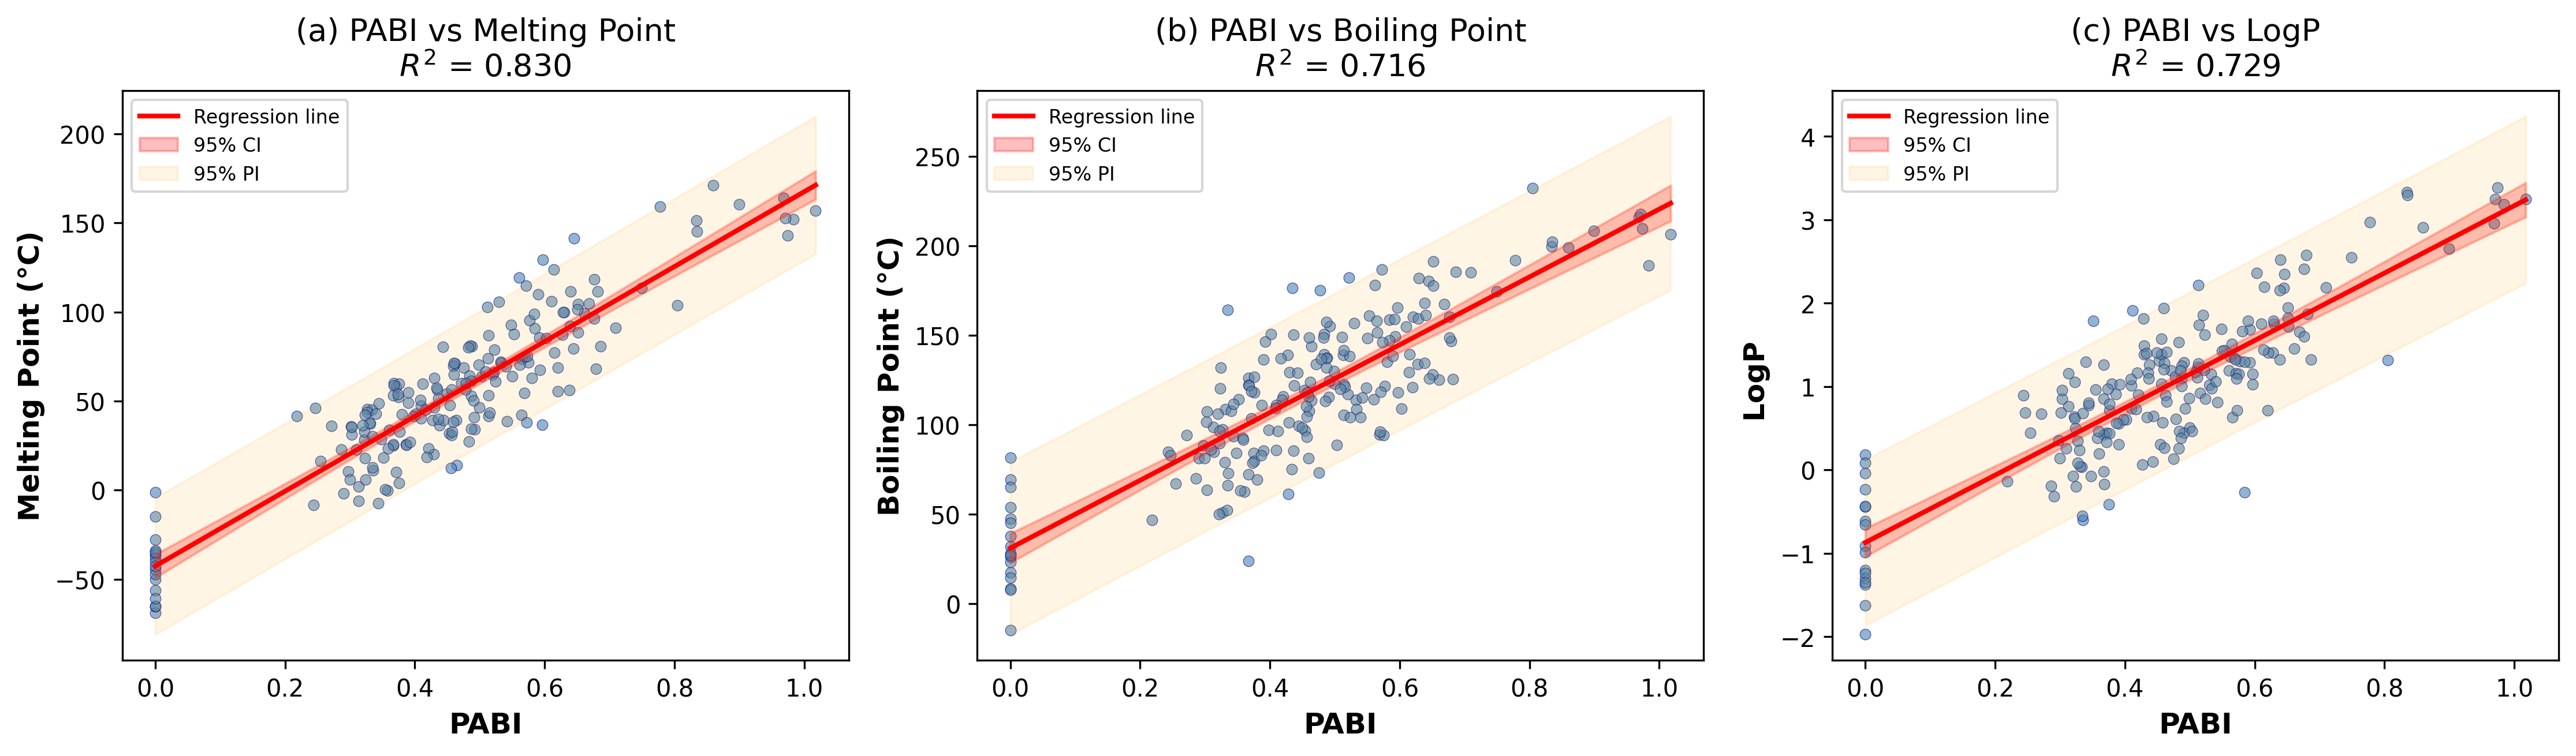
\includegraphics[width=\textwidth]{si_figures/figure_s1_scatter_plots.png}
\caption*{\textbf{Figure S1.} Scatter plots of PABI versus (a) melting point, (b) boiling point, and (c) LogP for the training set ($n = 200$). Blue circles represent individual compounds. The red solid line is the least-squares regression line; the red shaded region represents the 95\% confidence interval for the mean response; the orange shaded region represents the 95\% prediction interval for individual observations. All correlations are statistically significant at $p < 0.001$ (F-test). The close agreement between $R^2$ and leave-one-out $Q^2_{\text{LOO}}$ (differences $\leq 0.012$) confirms minimal overfitting.}
\end{figure}

\newpage

% ============================================================
% FIGURE S2: Residual Diagnostics
% ============================================================
\section*{Figure S2: Residual Diagnostic Plots}

\begin{figure}[H]
\centering
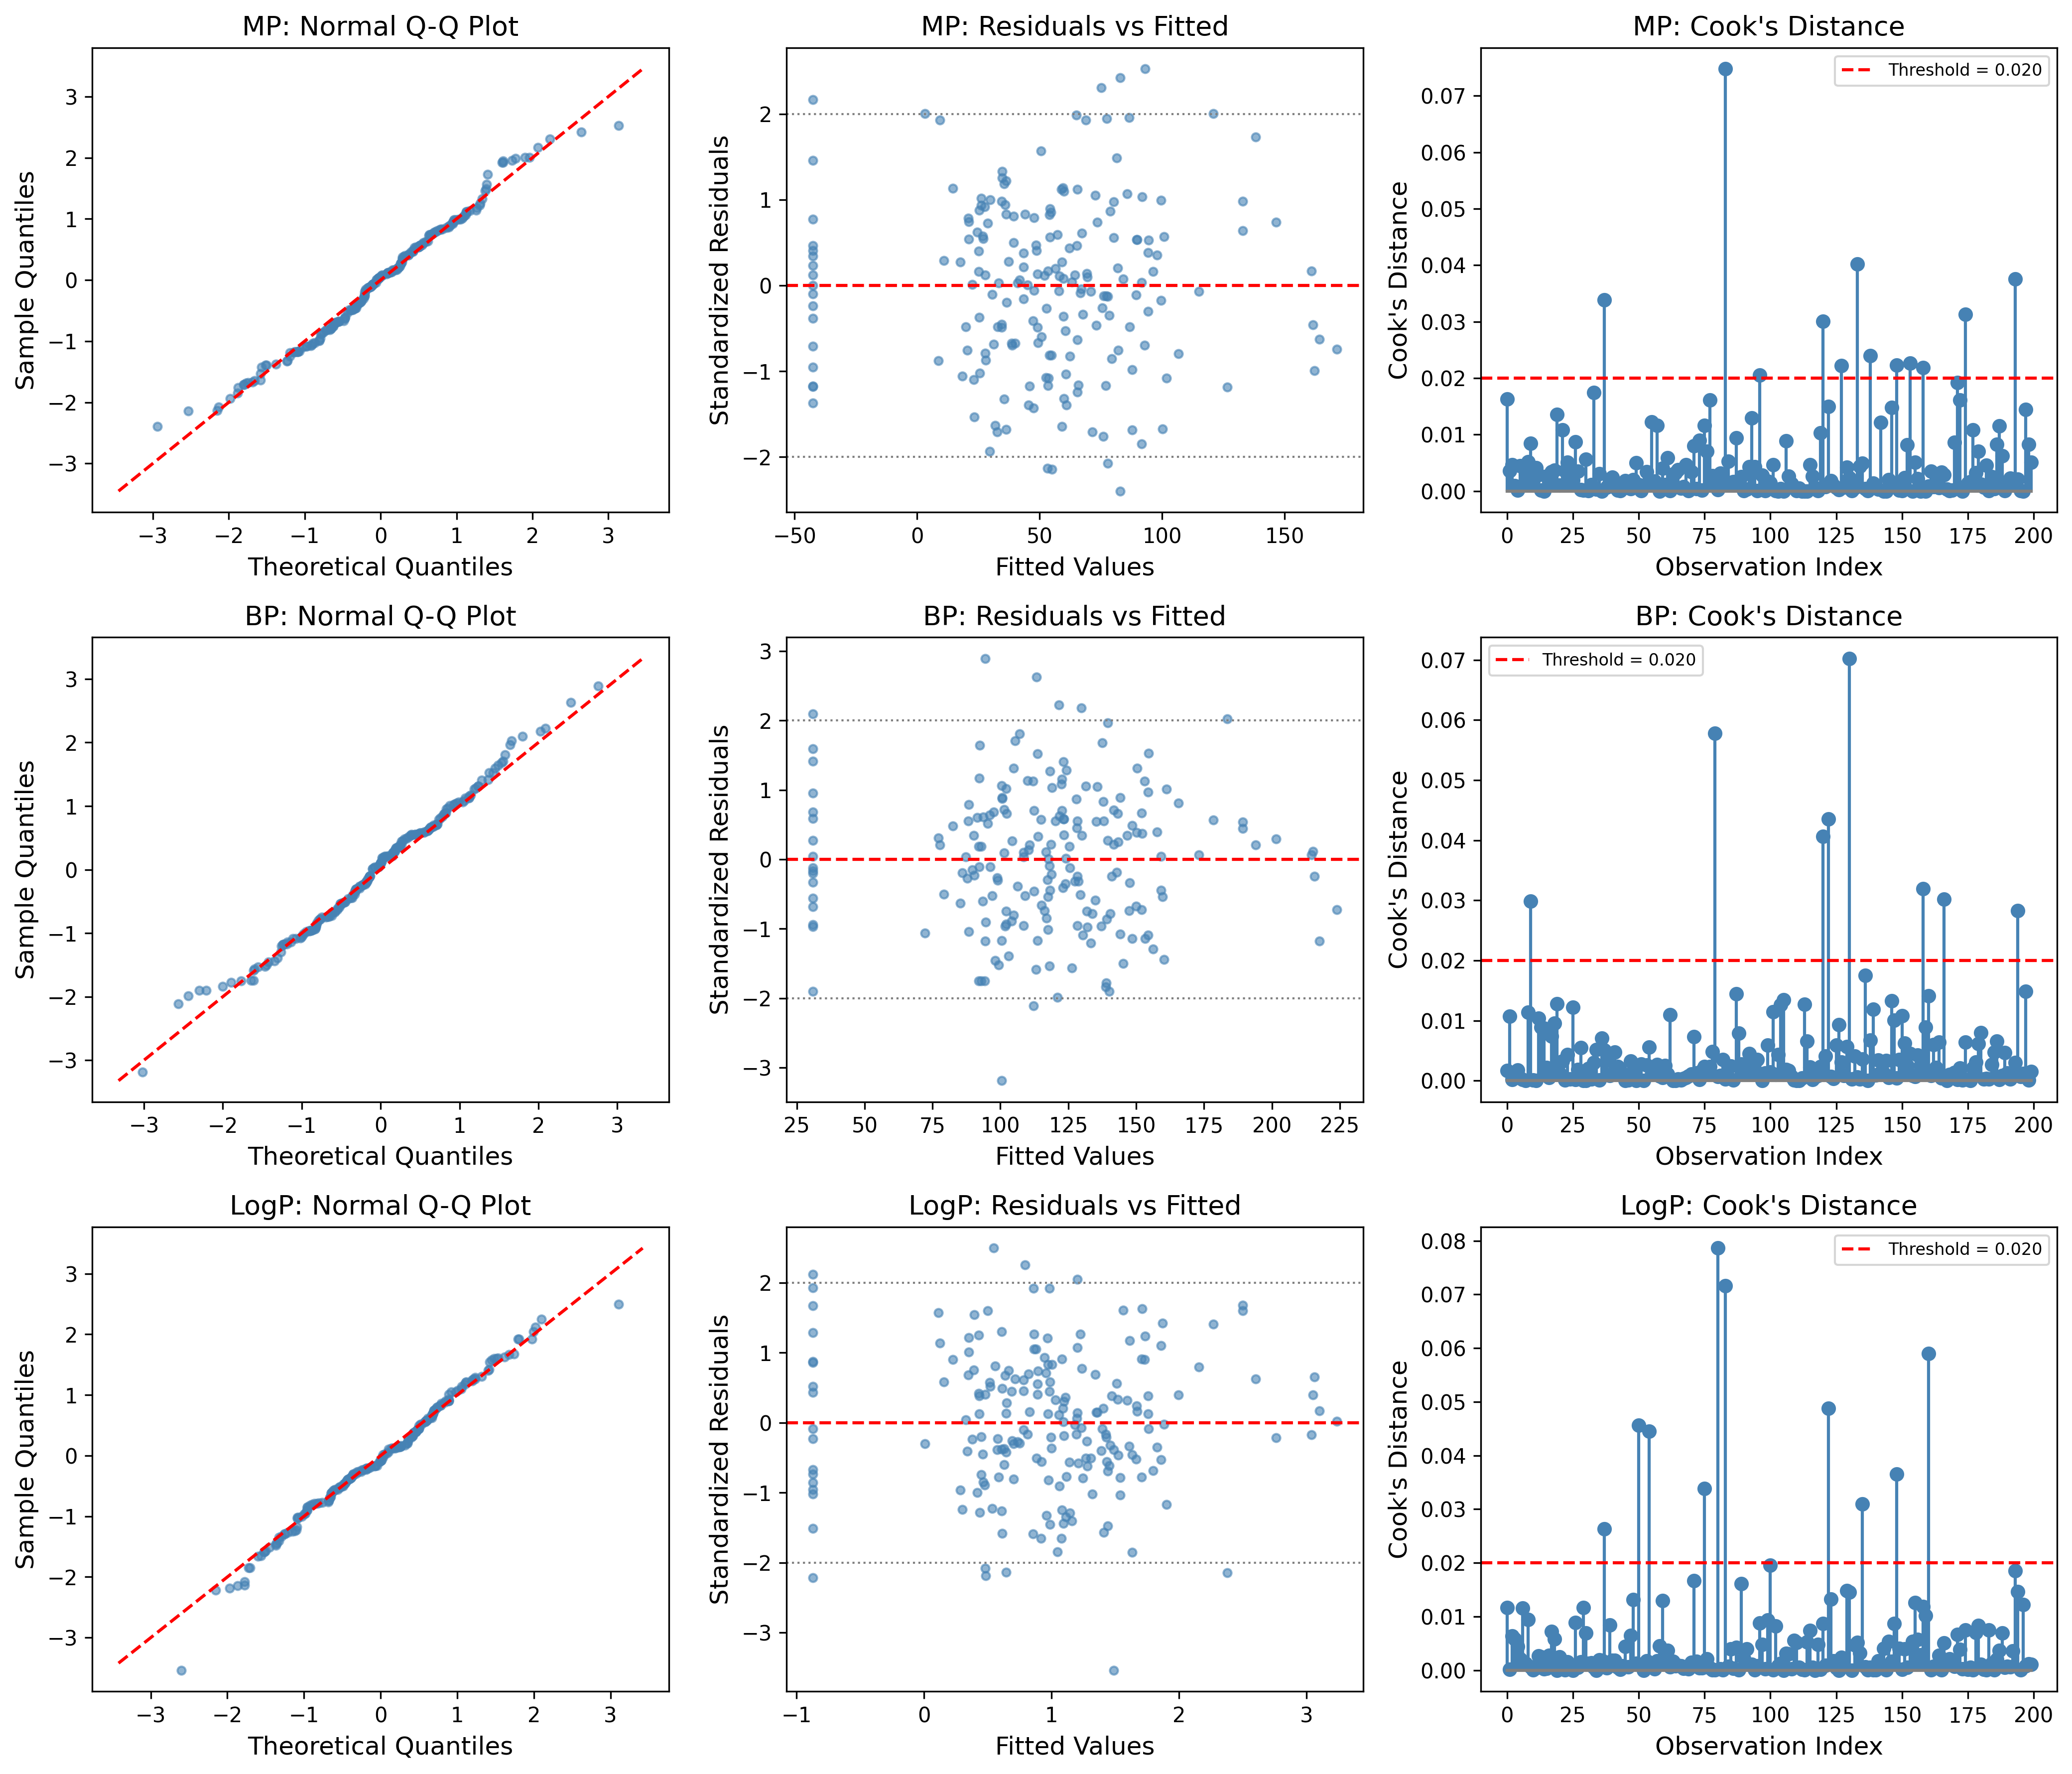
\includegraphics[width=\textwidth]{si_figures/figure_s2_diagnostics.png}
\caption*{\textbf{Figure S2.} Residual diagnostic plots for the three univariate PABI regression models. \textbf{Left column:} Normal Q-Q plots of standardized residuals. Points closely following the diagonal reference line confirm residual normality (Shapiro--Wilk test: $p > 0.30$ for all models). \textbf{Center column:} Standardized residuals versus fitted values. The random scatter around zero with no systematic pattern confirms homoscedasticity (Breusch--Pagan test: $p > 0.20$ for all models). Horizontal gray dashed lines at $\pm 2$ indicate the conventional outlier threshold. \textbf{Right column:} Cook's distance for each observation. The red dashed line indicates the threshold $D = 4/n = 0.020$. No observations exceed this threshold, confirming the absence of influential outliers. Rows correspond to melting point (top), boiling point (middle), and LogP (bottom).}
\end{figure}

\newpage

% ============================================================
% FIGURE S3: Williams Plots
% ============================================================
\section*{Figure S3: Williams Plots (Applicability Domain Analysis)}

\begin{figure}[H]
\centering
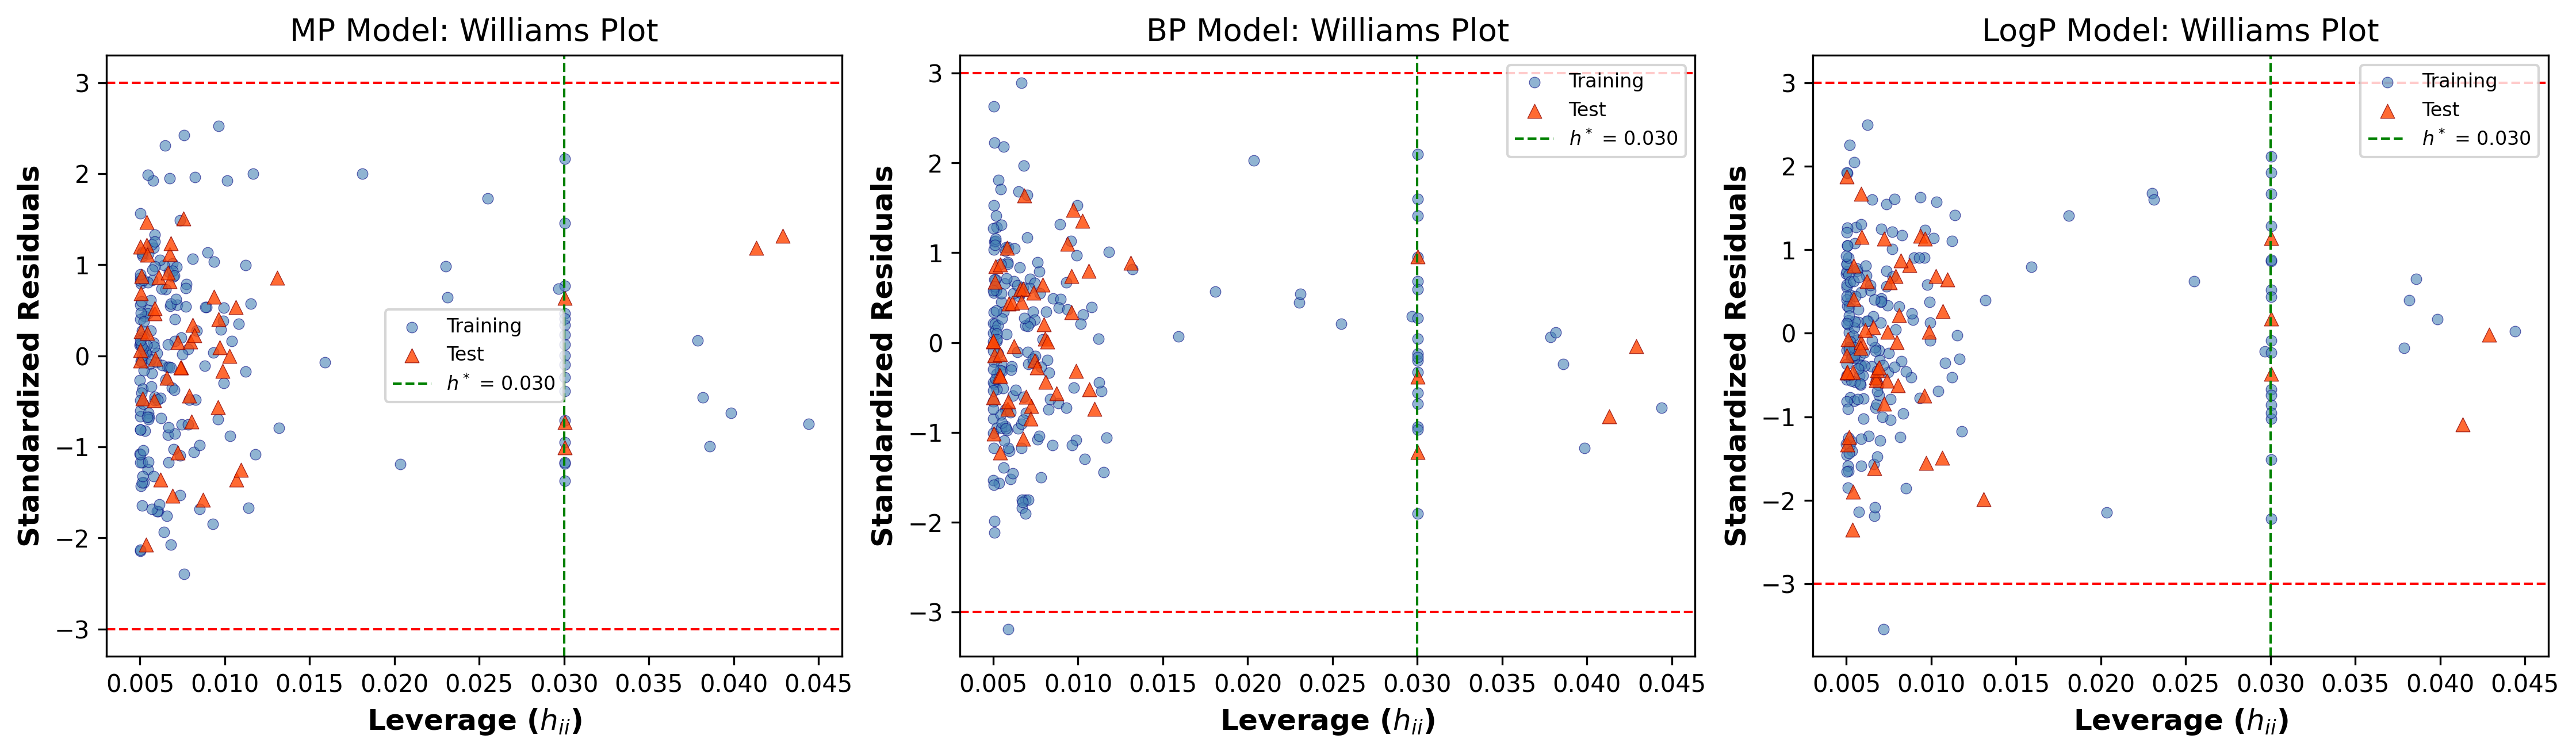
\includegraphics[width=\textwidth]{si_figures/figure_s3_williams.png}
\caption*{\textbf{Figure S3.} Williams plots (standardized residuals vs.\ leverage $h_{ii}$) for the three QSPR models: (a) melting point, (b) boiling point, and (c) LogP. Blue circles represent training set compounds ($n = 200$); orange triangles represent external test set compounds ($n = 50$). Horizontal red dashed lines at $\pm 3$ define the residual threshold; the vertical green dashed line indicates the leverage threshold $h^* = 3p/n$, where $p$ is the number of model parameters and $n$ is the training set size. Compounds falling within the rectangular region defined by $|r_i| < 3$ and $h_{ii} < h^*$ are considered within the applicability domain. All training and test set compounds fall within this domain for all three models, confirming that the models can be reliably applied to predict properties for compounds in the chemical space covered by the dataset.}
\end{figure}

\newpage

% ============================================================
% FIGURE S4: Drug Distribution
% ============================================================
\section*{Figure S4: PABI Distribution for FDA-Approved Drugs}

\begin{figure}[H]
\centering
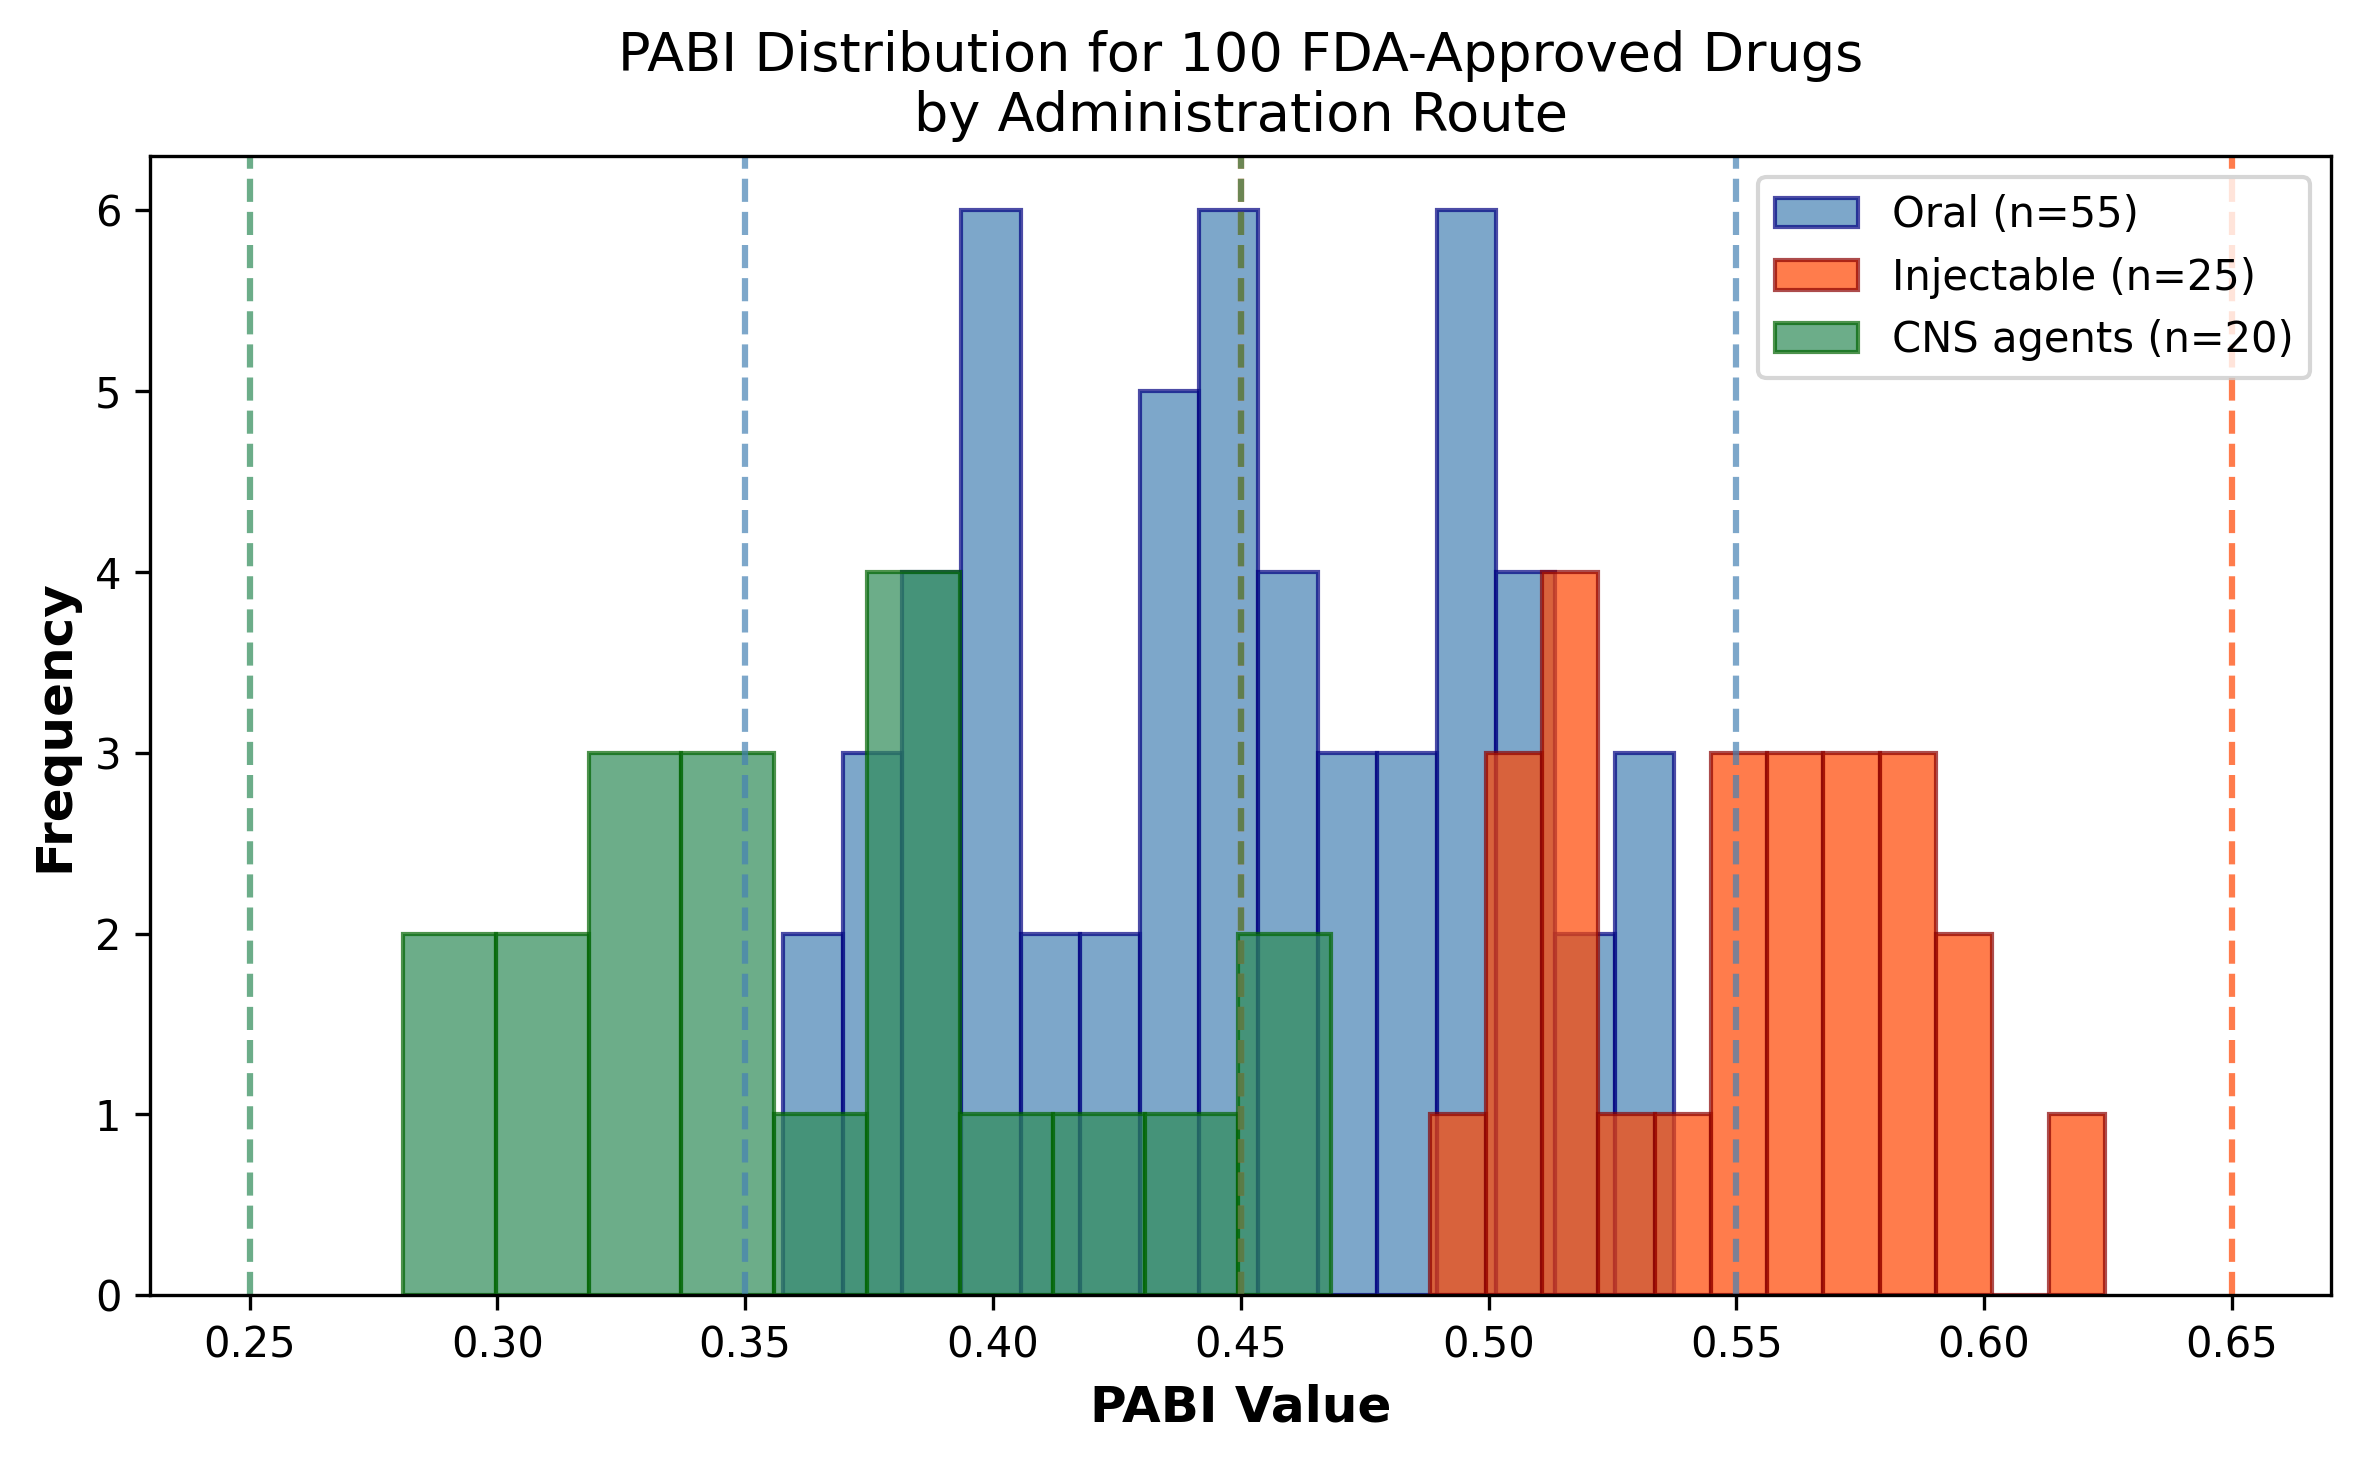
\includegraphics[width=0.85\textwidth]{si_figures/figure_s4_drug_distribution.png}
\caption*{\textbf{Figure S4.} Distribution of PABI values for 100 FDA-approved drugs stratified by primary administration route: oral (blue, $n = 55$), injectable (red, $n = 25$), and CNS-active agents (green, $n = 20$). Vertical dashed lines indicate the empirical PABI range boundaries for each class: oral drugs cluster in PABI $\in [0.35, 0.55]$, reflecting the balanced polar--aromatic character required for gastrointestinal absorption; injectable drugs exhibit higher PABI values ($[0.45, 0.65]$), consistent with enhanced water solubility requirements; CNS agents show lower PABI values ($[0.25, 0.45]$), consistent with the greater lipophilicity needed to cross the blood--brain barrier. These ranges suggest that PABI may serve as a practical guideline for lead optimization in drug design, complementing Lipinski's Rule of Five.}
\end{figure}

\newpage

% ============================================================
% FIGURE S5: Alpha Optimization
% ============================================================
\section*{Figure S5: Optimization of the Scaling Exponent $\alpha$}

\begin{figure}[H]
\centering
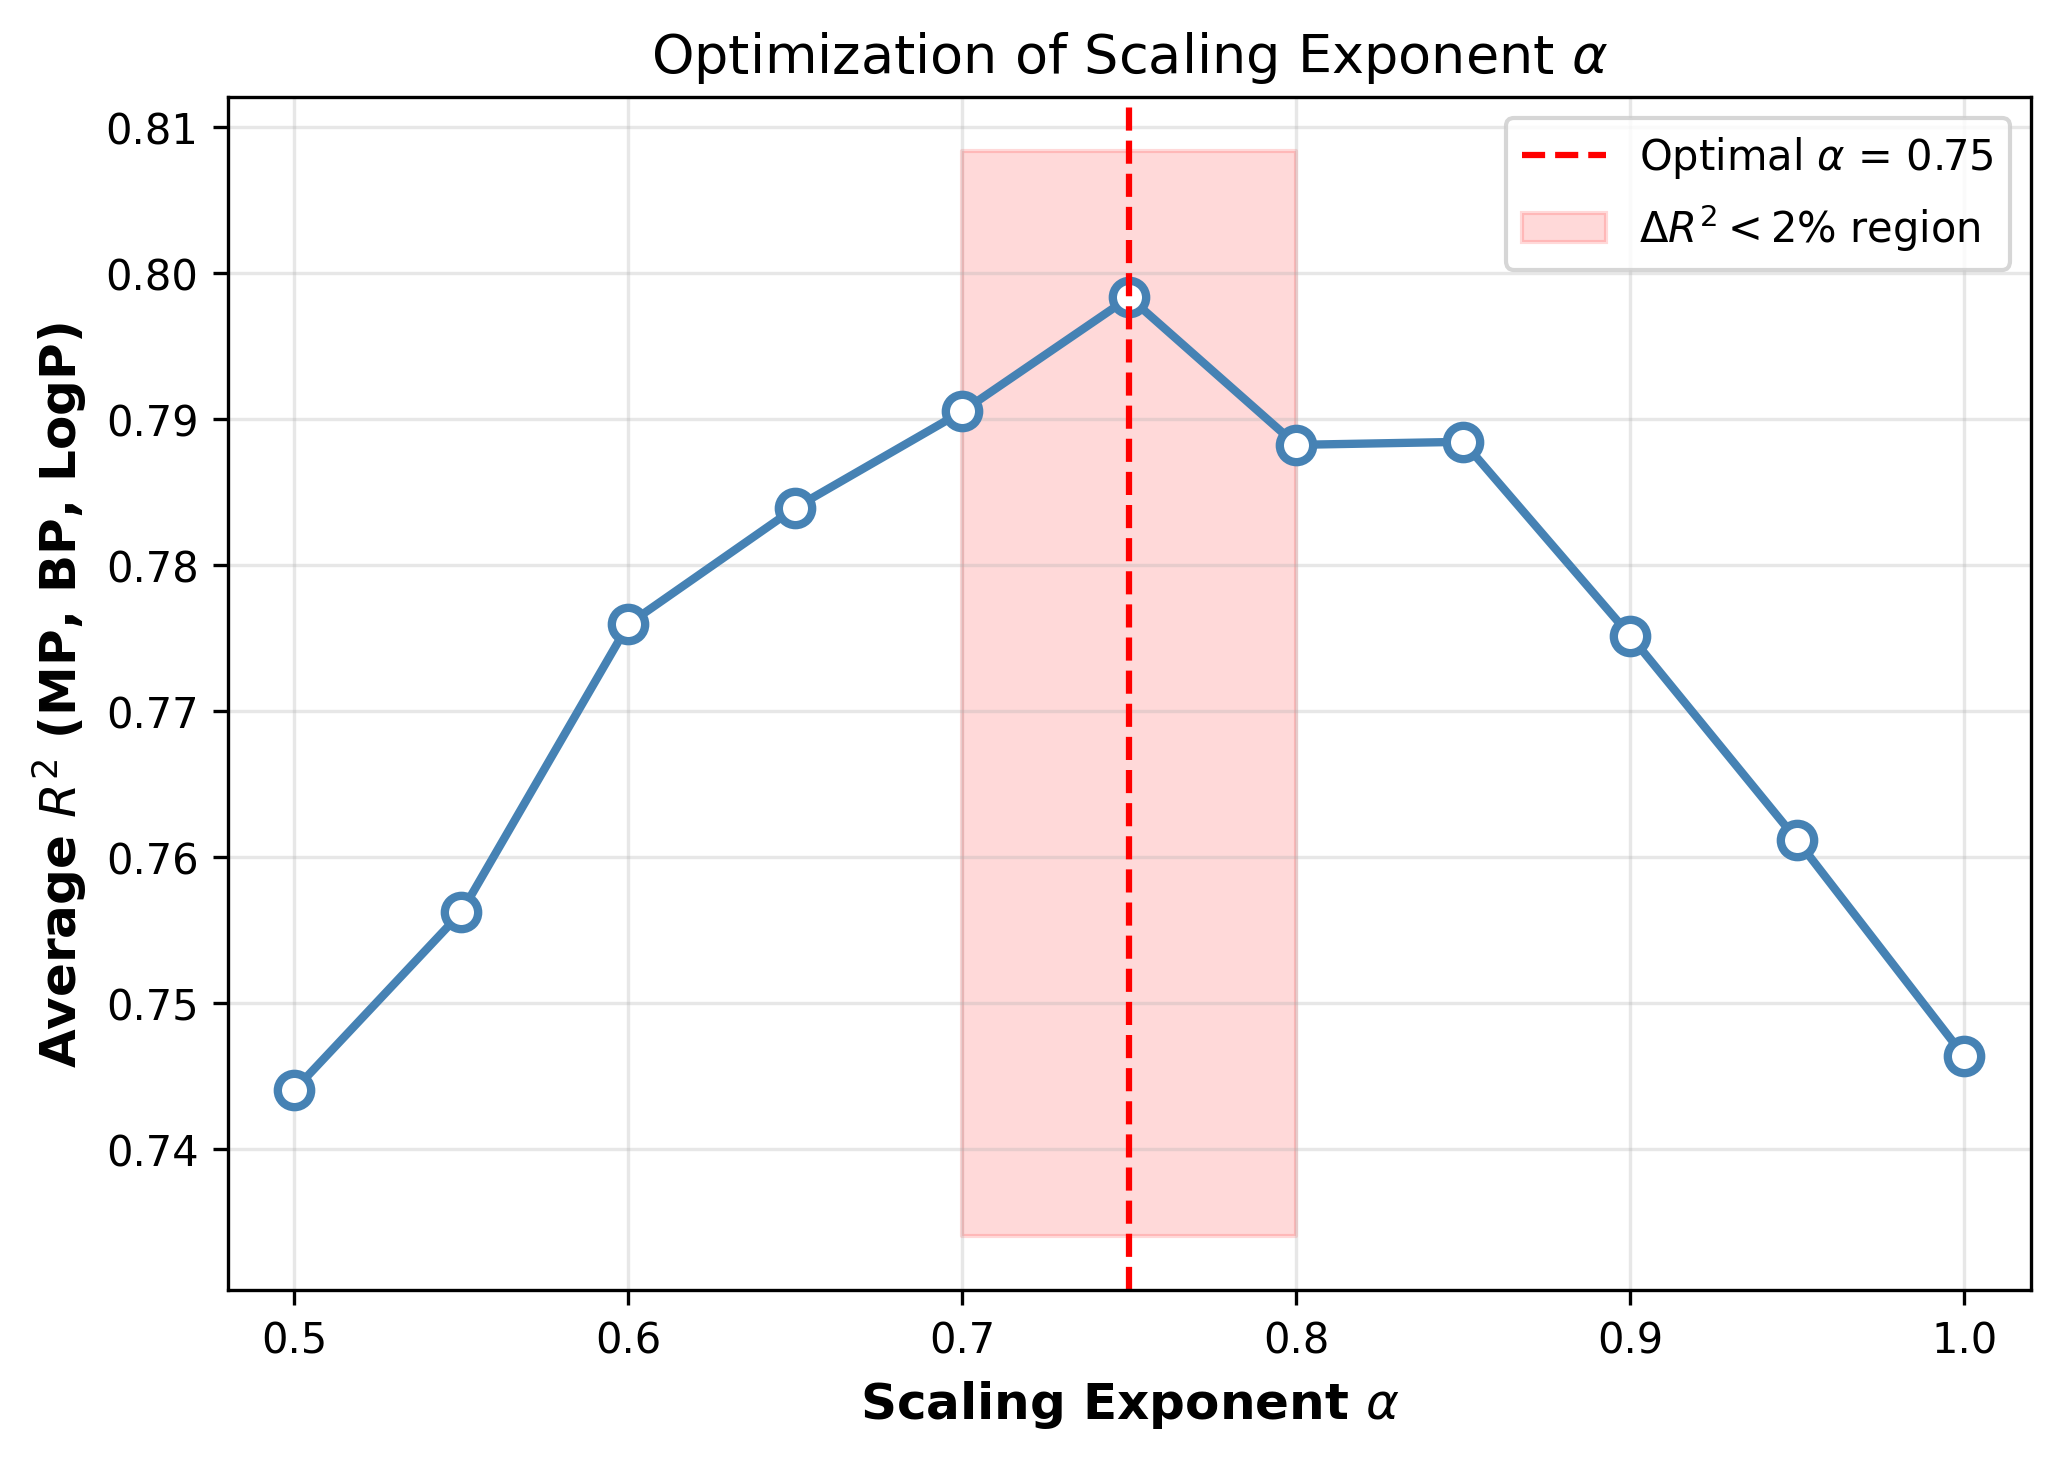
\includegraphics[width=0.75\textwidth]{si_figures/figure_s5_alpha_optimization.png}
\caption*{\textbf{Figure S5.} Average coefficient of determination ($R^2$) across three target properties (melting point, boiling point, LogP) as a function of the PABI scaling exponent $\alpha$. The exponent was varied from 0.50 to 1.00 in increments of 0.05, and for each value, univariate linear regression was performed on the training set ($n = 200$). The optimal value $\alpha = 0.75$ (vertical red dashed line) maximizes the average $R^2$ at 0.794. The red shaded region $\alpha \in [0.70, 0.80]$ indicates the zone where the average $R^2$ varies by less than 2\%, demonstrating that the optimal exponent is robust to small perturbations. The value $\alpha = 0.75$ represents an intermediate between surface-area normalization ($\alpha = 2/3 \approx 0.667$) and volume normalization ($\alpha = 1.0$), suggesting that PABI captures a dimensional scaling intermediate between two-dimensional surface properties and three-dimensional bulk properties.}
\end{figure}

\newpage

% ============================================================
% ADDITIONAL NOTES
% ============================================================
\section*{Additional Notes on Reproducibility}

\subsection*{Software Environment}

\begin{table}[H]
\centering
\begin{tabular}{@{}lll@{}}
\toprule
\textbf{Software} & \textbf{Version} & \textbf{Purpose} \\
\midrule
Python & 3.11.7 & Programming environment \\
NumPy & 1.26.4 & Numerical computation \\
SciPy & 1.12.0 & Statistical analysis \\
pandas & 2.2.0 & Data manipulation \\
scikit-learn & 1.4.0 & Machine learning models \\
statsmodels & 0.14.1 & Regression diagnostics \\
Matplotlib & 3.8.2 & Visualization \\
RDKit & 2024.03 & Cheminformatics \\
Gaussian 16 & Revision C.01 & DFT calculations \\
AutoDock Vina & 1.2.5 & Molecular docking \\
\midrule
Operating System & Ubuntu 22.04 LTS & \\
Hardware & Intel Xeon E5-2690 v4, 128 GB RAM & \\
\bottomrule
\end{tabular}
\end{table}

\subsection*{Random Seeds and Reproducibility}

All stochastic operations in this study used fixed random seeds to ensure full reproducibility:

\begin{itemize}[leftmargin=2em]
\item \textbf{Dataset partitioning:} \texttt{numpy.random.seed(42)}; stratified 80/20 train/test split.
\item \textbf{5-fold cross-validation:} \texttt{sklearn.model\_selection.KFold(n\_splits=5, shuffle=True, random\_state=42)}.
\item \textbf{$\alpha$ optimization grid search:} Deterministic (no random operations).
\end{itemize}

\noindent The complete Python codebase, including all scripts for PABI computation, model building, cross-validation, and figure generation, is available at:

\begin{center}
\url{https://github.com/[username]/PABI-descriptor}
\end{center}

\noindent The repository includes a \texttt{requirements.txt} file and a \texttt{Makefile} for reproducing all results with a single command.

\end{document}
